\section{Process}
\subsection{Methodology}
\begin{itemize}
    \item Meetings
    \item Extreme programming
    \item Evaluation Criteria (How were they defined)
\end{itemize}

\subsection{Communication}
Communication with Vixel was done through biweekly status meetings, where they would be briefed on progress, and answer any questions we had related to the direction of the project. Additionally, we would sit in their office when working with the project, allowing for easy communication. Any communication outside of these situations happened through Slack.

\subsection{Pair Programming}
Throughout the project we adopted a pair programming methodology. This was done to ensure that both group members were familiar with the functionality of the code, and to allow us to quickly exchange ideas as to how the functionality could be implemented.

\subsection{High-level Architecture}
\subsubsection{Vixel Proposed Architecture}
Vixel was quite clear on what solution they desired, and presented us with a proposed architecture, seen in Figure~\ref{fig:proposed_architecture}. In their proposed architecture the images captured by the camera is sent to a distribution server. From here the video feed is distributed to an clients who \rephrase{are listening for it.}
In the case where a client user clicks to highlight something on their screen, that interaction request is sent to the host through the distribution server.


\begin{figure}
    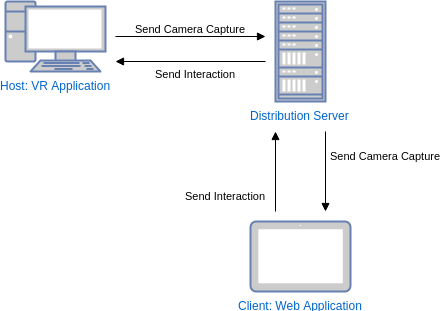
\includegraphics[width=0.8\textwidth]{vixel_stream}
    \caption{Proposed architecture by Vixel}
    \label{fig:proposed_architecture}
\end{figure}

\subsubsection{Our Architecture}
Our final solution is kept quite close to the original solution, with some minor differences. As seen in Figure~\ref{fig:our_architecture} rather than only having one distribution server, two cloud servers are used to achieve the desired functionality. The video stream captured by the camera in the host VR application is sent to a dedicated streaming platform, rather than the distribution server. Interactions between the client and the VR application, such as highlighting, is handled through the Photon Cloud. With the move to a dedicated streaming platforms, the client needs to know where to watch the stream. The URL for this stream is also communicated through Photon Cloud.

\paragraph{Justification}
Splitting the distribution server into two separate pieces allowed us to better focus on combining existing solutions to allow us to get a functioning proof of concept faster. Having a distribution server would require us to set up a basic streaming platform. The distribution server would also need functionality to allow it to speak to both the host side Unity VR application and the client web application. Such a solution would require us to satisfy potentially complex networking protocols. This was something we neither had time, nor competence to do.

\begin{figure}
    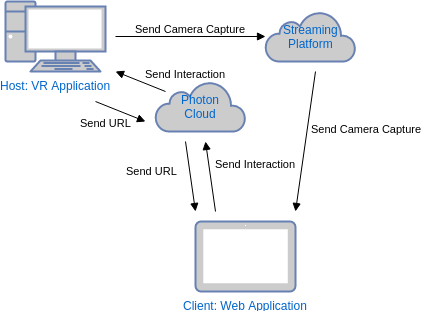
\includegraphics[width=0.8\textwidth]{our_stream}
    \caption{Final Architecture}
    \label{fig:our_architecture}
\end{figure}

\subsection{Technology Assessment and Component Architecture}
As part of developing the component architecture we had to assess a large array of various technologies to best satisfy Vixel's requirements. This section contains the assessment framework we used, a brief description of each alternative we looked at, its strengths and weaknesses as well as our final choice of technology.  

\subsubsection{Assessment Framework}
Our assessment framework consisted of a two-step process. To start off, we had to gauge our first impressions on the various types of technology that exists. We handled this by setting up a list of criteria for each component where each had an importance multiplier between 1 and 5 where higher values means higher importance. The list of criteria included aspects like performance, potential expenses, existing familiarity, documentation, reliability as well as a few others. We gave each technology a score between 0 and 9 where higher means better and combined the score with the importance multiplier for each criteria. We would then consider the technologies that ended up with the highest sum of criteria scores for potential prototyping as well as the final choice. 

While we have assessed a variety of different technologies, we acknowledge that we may have missed some which might have been relevant for the project. We also handled the assessment with the original architecture in mind, but the final architecture ended up being slightly different as we had become more familiar with the topic. Our final choice of technologies also had some influence on the final architecture. 

\subsubsection{Host - Image Capture} % FFMPEGOut in combination with FFMPEG. Some modified source code for optimization and repurposing for streaming
Image capturing is a subcomponent of the host component where the goal is to capture images at a set time interval from a camera that exists in Unity. The captured images then need to be encoded to a video format in order for streaming to be possible. As far as technology assessment is concerned, we primarily looked at the actual problem of capturing images first and foremost as it was the most pressing issue in relation to performance. The solution alternatives we looked at are as follows:

\paragraph{Native C++ Plugin, using OpenGL access to acquire framebuffer}
Unity has support for native plugins\cite{unity_native_plugin} which allows us to write code in native C++ through the use of .DLL files. The use of native plugins gives full access to Unity's rendering pipeline which we could have used to access the framebuffer directly for image data acquisition. The strength of this approach is that it provides a large amount of control which in turn could provide a high performance potential. On the other side there are a couple of weaknesses with this approach. This includes the need to restart Unity every time we want to reload the plugin, a higher degree of code complexity by using C++ and the need to intimately understand Unity's rendering pipeline.  

\paragraph{RockVR Video Capture}
RockVR Video Capture\cite{unity_asset_store_rockvr} is a free plugin on the Unity Asset Store that allows for plug and play video capture functionality. The primary benefit of this solution is the simplicity of setting the plugin up and using it to capture video. As far as weaknesses are concerned we tried to write a quick prototype using the software, but noticed that the performance was insufficient as the plugin forced a vertical synchronization on the rendering itself. We also found it hard to understand whether it was possible to replace the encoding to video file with a real time encoding that could be directly transferred instead of saving the data locally on the machine first. Other weaknesses includes the fact that the licensing of the plugin was unknown and that usage of more advanced functionality required a paid version. 

\paragraph{Naive implementation using the RenderTexture component in Unity}
The perhaps simplest solution would be to write a naive implementation using the RenderTexture\cite{unity_renderTexture} component in Unity to directly copy pixel data from a camera to a texture. The benefits of this approach is that the implementation is very easy to prototype and that the code complexity is fairly low. On the other hand, the simplicity of the solution severely impacts performance.  

\paragraph{Optimized Naive implementation}
While searching for alternatives we managed to find a blog post\cite{google_vrCaptureBlog} by one of the Google's Tiltbrush developers which discusses an optimized version of the previously mentioned naive implementation. The blog post specifically mentions that several optimizations could be made to allow for real-time VR video capture in Unity. It could therefore be possible to create an optimized naive implementation as long as it is possible to retrace the steps that the blog post goes through. The strength of this approach is that it should provide high enough performance for video capture in real time if the author is to be believed. The downside is that the solution is described at a rather high level which can make it hard to actually implement everything as we have limited knowledge on the topic. 

\paragraph{Unity Generic Frame Recorder}
Unity offers a open source video capture plugin\cite{unity_genericFrameRecprder} which contains a large amount of various functionality. The benefits of this plugin is that it seems to be fairly large and extensible as it is made by Unity Technologies, the code is fairly well documented and it is also open source. The downside is that the codebase is rather big and complex. This can make it hard to actually modify and extend the code to fit our needs. A quick test of the plugin also makes it seem like the performance is not satisfactory to fulfill Requirement~\ref{req:minimal_processing_host}.

\paragraph{Using the AsyncGPUReadback from the latest Unity version}
Unity version 2018.1 and onwards has added the possibility of asynchronous readback from the GPU\cite{unity_asyncReadback} which in theory should allow for high performance fetching of GPU data. Using this functionality should avoid stalling the rendering pipeline in the way that RenderTexture components do which in general should provide better performance. The problem with this approach is that the technology is experimental and may be removed in later versions. There are also no actual open source implementations at the present time that handle video recording in a high performance manner. We attempted to write a quick prototype using the technology, but ended up with lower performance than the naive RenderTexture implementation. The reason for this is that we could not find an efficient means of converting the data we received from the GPU do a format that would be acceptable for encoding. 

\paragraph{FFmpegOut}
The final alternative we looked at is FFmpegOut\cite{ffmpegOut} which is a open source plugin for Unity that takes care of video recording using the FFmpeg\cite{ffmpeg} library. This solution had several strengths. From all the alternatives we looked at, this plugin provided the best performance in terms of actual video recording. It also gives full access to FFmpeg library which can handle both video encoding and video streaming. The code itself is open source and the codebase is small which should make potential optimizations and changes very easy to keep track of. There are also two downsides with this solution. The first is that it requires time to learn the FFmpeg library to be able to modify and extend of source code for our purposes. The second is that the pipe that the source code uses to FFmpeg is not perfectly robust as recording might suddenly stop working if the application window is not in focus for a few seconds.  

\paragraph{Final Choice of Solution}
Given that performance was a priority for this component, we prototyped all of the already made solutions in combination with the implementation of the simple naive approach. In general, the majority of the solutions had many oddities that impacted the performance in a negative manner like forcing the framerate of the application to be the same as the recording. Furthermore, many of the solutions saved data to video files, which is not needed for our case as we want to take the encoded data and stream it in real time without the intermediary step of saving the data to disk. We finally chose FFmpegOut as it also allowed us to handle real time video encoding of raw image data and stream it using the RTMP protocol. This meant that FFmpeg could fill the role of the data transfer that was needed for the host component. It also had the best performance among the alternatives even if it was not optimal. The fact that the code was open source also allowed us to easily modify the code to suit our needs. Since video encoding is handled by FFmpeg we also did not have to spend additional time to implement this ourselves. 

For the final solution we use a modified version of FFmpegOut. In this modified version, we have optimized the performance so that it no longer forces vertical synchronization by modifying the camera capture algorithm to sample the camera at set time intervals instead of every frame. Instead of encoding and saving the raw image data to a video file, we have also entirely replaced the FFmpeg command arguments to allow for streaming to servers that support the RTMP protocol. 
    
%%%%%%% Note: If we are to cut anything: we can technically cut a large amount of this as we mentioned that FFMPEG Handles Data Transfer
\subsubsection{Host - Data Transfer} % FFMPEG
Data Transfer is another subcomponent of the host side where the main goal is to take the encoded video data and stream it to a distribution server. For this subcomponent we considered the following solutions:

\paragraph{Native C++ Plugin Using Boost}
Similar to the actual image capture, we considered using a native C++ plugin for Unity. In this case we would have been using the networking components of the Boost library\cite{boost} to transfer data to the distribution server. Using Boost would allow us to have full access to sockets which gives a lot of control. At the same time, this means that we would have to make our own protocols which would take time. Boost is also a big library which can result in lengthy compilation times. The fact that Unity needs to be restarted to reload the plugin is also a downside. 

\paragraph{Unity's Transport Layer}
While Unity offers a high level network API which is primarily focused around networking for games, it also offers a lower level API called the Unity Transport Layer\cite{unity_transportLayer}. This API should provide enough functionality to facilitate the process of data transfer to a distribution server without the need for any additional dependencies. In general, the reliability of this component of the Unity engine should also be fairly solid as all of Unity's networking functionality is built on top of it. The main problems with this API is that the documentation in general is not particularly comprehensive, that we would probably have to write our own data transfer protocols and the fact that we have limited familiarity with the technology which makes it hard to prototype with as the complexity is somewhat high. 

\paragraph{Photon Engine}
The Photon Engine\cite{photon_homepage} offers a Unity API for networking which we potentially could use for transferring data as it supports communication between many different platforms. The benefits of using the Photon Engine would be that later integration might be easier as Vixel already makes use of it. The Unity API is also fairly simple and well documented which should make it easy to prototype and implement functionality. Finally, it would allow us to use the same technology in multiple components regardless of platform as the engine supports many programming languages and platforms. A weakness of this solution is that it is not really built for transfer of video data, but rather smaller game state communication. The solution can also become expensive in order to get satisfactory performance from the provided cloud servers. 

\paragraph{FFmpeg}
FFmpeg was already mentioned when listing alternatives for the previous subcomponent of the host side, but is again relevant here as it is related to this area as well. The benefit of using FFmpeg for data transfer is that it directly supports the RTMP protocol which is standard for video streaming. The library is also very mature and well documented which means that finding the necessary information for our goals should be fairly easy. The downside is the same as already mentioned in relation to the fact that the library is rather large so properly understanding it can take some time. 

\paragraph{Final Choice of Solution}
In general, it was hard to make a choice for this component as we had very limited prior experience with large scale data transfer. We had originally planned to try the Unity Transport Layer for data transfer as it would reduce the the overhead of working with additional technologies. We also considered trying the Photon Engine, but discussion with Vixel provided us with the information that Photon is not particularly efficient at transferring large amounts of data like video streams. We ultimately chose FFmpeg for data transfer as it already was used for video encoding. An additional benefit of choosing FFmpeg was that prototyping the solution took less time as FFmpeg could take care of several things for us which is very valuable when limited time is available. Since FFmpeg primarily is focused around working with video files it is also a very optimized library for this purpose, which is perfect for Requirement~\ref{req:minimal_latency} where minimal latency is preferred. 

\subsubsection{Host/Client Communication} % Photon
This component consists of facilitating the communication between the clients and the host. This includes distributing stream URLs from the host and the interaction from the client side to click on things they see in the stream. In general, the aforementioned alternative solutions for data transfer are relevant for communication although there are some exceptions. Since the client will be hosted on a web page, we need to make sure that cross technology and cross platform support is possible. This excludes the use of a native C++ plugin with Boost as it cannot easily interact with a Javascript web page. FFmpeg is also not relevant for this purpose as it only works with video files.  
    
\paragraph{Unity's Transport Layer}
Using the Unity Transport Layer API would in general give us a lot of control in terms of how communication is handled, but the general complexity of networking at the lower level may be too high for the simple communication between clients and host. Using the Transport Layer API could also potentially force us to use Unity on the client side which might result in a less maintainable and extensible solution. Ideally, we would prefer to have all the components as interchangeable as possible. 
      
\paragraph{Photon Engine}
The other option is to use Photon for the communication between host and clients. The benefit of using Photon is that it is very easy to set up for the simple communication purposes we need and that it has full cross platform and cross technology support which allows a the C\# side of Unity to communicate with a Javascript side where both use Photon. The only downside of using Photon for this is that the free plan has somewhat limited functionality, although it should not be a limitation for a prototype. 

\paragraph{Final Choice of Solution}
We ultimately went with Photon for communication as it was easy to set up for prototyping and because it allowed for better interchangeability between components, giving us more freedom to make the client side however we wanted. 
    
    
    
    
    
    
    
    
    
    
    
    
    
    
    
    

\subsubsection{Server - Stream Distribution} % Youtube, Twitch, Mixer, Self made streaming solution
The encoded video data from the host needs to be distributed to all the clients. To avoid additional use of bandwith and computation on the host, a distribution server was desired. Additionally, as noted in requirement \ref{req:minimal_latency}, we wanted as low latency between the host upload and clients download as possible, as to not disrupt the user experience. We saw three main alternatives when assessing this technological choice, a self-made streaming platform, using existing streaming middleware, or using existing streaming platforms like YouTube or Twitch.

    % * The encoded video data needs to be sent to a type of distribution server which takes the data and streams/distributes it to all connected clients in the form of a livestream.
    %     * Because the host should not be using additional bandwidth other than sending the video data to this server. 
    
\paragraph{Self-Made streaming platform}
A self-made streaming platform would give us total control over the component, allowing us to tweak whatever options we desired to decrease potential overhead. However, such a solution would require us to host the server ourselves, and the bandwidth throughput would be heavily affected by what deals we would get with our local internet service providers. Additionally, trying to create a streaming platform from scratch with no prior experience during the time available to us would be unrealistic at best.

    % * Description
    %     * As the name implies, this solution would require us to make our own streaming platform which distributes the stream data to all clients. 
    % * Strengths
    %     * Full control over this component of the solution
    %     * Potentially no expenses
    % * Weaknesses
    %     * We will have to host the server locally which limits bandwidth throughput
    %     * Complexity of creating a streaming platform from scratch without any prior experience is very large. 
\paragraph{Making use of existing stream middleware}
    * Description
        * There is streaming middleware out there which could be used to create our own streaming platform in a quicker manner. \todo{add examples}
    * Strengths
        * Potential cloud distribution should make bandwidth less of a problem.
        * A fair amount of control is still given in relation to how the server distributes streaming. 
    * Weaknesses
        * There are usually expenses involved in both the platform and cloud hosting.
        * Unknown latency between host and client. 
\paragraph{Making use of streaming platforms like Youtube and Twitch}
    * Description
        * The final alternative would be to make use of existing streaming platforms like Youtube/Twitch and embed their stream player into our website with input functionality overlayed on top of the player. 
    * Strengths
        * Completely free
        * High performance distribution of streams which should result in minimal latency
        * Easier and faster to prototype with
    * Weaknesses
        * Technically using the platforms for purposes they are not made for.
            * Point 5.G in the youtube terms. 
                * Not sure if we are breaking this rule, but we are blocking the possibility of pausing the stream.  
                * And we are building functionality on top of it.
                * Move this to final choice of solution and say: In retrospect we
        * Very limited control over the platform. 
\paragraph{Final Choice of Solution}
    * Our final choice here ultimately ended up being using Twitch and Youtube as our streaming platforms. The rationale behind the choice is
        * we simply did not have the time and resources available to make our own streaming platform
        * we do not want to spend money on the solution for a prototype
        * latency is of high importance so we went with the best free solution that also provided the minimal latency. 
    * The loosely coupled architecture of the project makes it easy to potentially replace what we used with another platform.






















\subsubsection{Client} % Unity Overlay HTML 5, Moving to pure javascript, Remember: glorious html overlay hack
The client component is responsible for playing the livestream video, while also listening for mouse clicks, which are sent back to the host.
Due to the requirement\reqref{req:no_client_software} of not installing any software on the client, our options for creating the client application was quite limited. 
To comply with the requirement we choose to create a web application, however, we identified some alternatives as to how we could best achieve the desired functionality.

\paragraph{Pure Javascript Client}
An obvious solution for the client application is to create it in plain javascript. Javascript would allow us to play videos with embedded links, and register mouse input from the user. Creating the client in pure javascript would ensure cross platform compatibility in a lightweight manner. However, there are some disadvantages to this approach. Photon supplied javascript support, however, cross-platform communication with Unity applications does not come right out of the box\cite{photon_javascript}, and their documentation on the javascript API leaves a lot to be desired. Additionally, neither of us are particularly well versed in javascript, which would decrease our prototyping productivity. 

\paragraph{Unity WebGL}
Unity has support for creating HTML5 applications using WebGL\cite{unity_webgl}, through the translation of C\# and UnityScript code to Javascript. Unity was quite desirable for us, it would allow us to not only have the same technology from host to client, reducing complexity, but also allow for fast prototyping as we were familiar with the technology. 
However, Unity WebGL also brings some challenges. Unity WebGL support is lacking in several aspects, with builds that are prone to fail randomly, or take a long time. While WebGL on mobile and tablet devices are not directly supported by Unity, Unity Technologies state in their documentation that high-end devices might be able to run WebGL applications. Due to the low level of computation required by our client application, we think it would be possible to run it on a mobile or tablet device. However, how well the application runs on a mobile or tablet device is unknown. Additionally, Unity is a heavy solution for the problem we are trying to solve.
Using Unity would handle the problem of registering input and communicating with the host. However, we would still need to display the video stream coming from the host. Several solutions was investigated to solve this problem.

\subparagraph{Video Player Component}
Unity's video player component allows for playback of videos, by rendering the video onto the texture of a game object\cite{unity_video_player}. The video player component has support for streaming videos from an URL. However, this has to be the direct video URL, meaning that a regular YouTube URL would need to be decoded to get access to the actual video feed, before it could be supplied to the video player component. Additionally, it is uncertain if such a solution would go against YouTube's guidelines\cite[5.1 A]{youtube_guidelines}.

\subparagraph{YouTube Player (Asset Store)}
Several YouTube video player solutions exist within the Unity ecosystem. However, we were unable to find any free solutions that also guaranteed cross platform support. 

\subparagraph{In App Browser}
Another alternative would be to create a browser within Unity\cite{unity_simple_browser}. Such a browser would easily integrate with whatever streaming platform that was chosen, however, it was only supported on windows, and would have been quite a heavy solution.

\subparagraph{WebGL Overlay Over Iframe}
\todo{Rephrase most of this!}
A fourth solution is to make the WebGL application transparent and place it on top of a video player. Such a solution is possible as Unity supports interacting with browser scripting through javascript\cite{unity_webgl_javascript_interaction}, allowing us to modify the HTML document the WebGL application is deployed in. 
This allows Unity to take care of the input handling, and communication with the host, while the video stream is handled by an iframe video player. A benefit of this approach is the louse coupling to the streaming service it creates, as it only requires an embeddable iframe link to where the video stream is.

    
% \paragraph{HTML5 Youtube Player With Unity WebGL Overlay}
%     * Description
%         * Another option is to have a Unity interface as the overlay over the stream player. 
%         * Using Javascript plugins for Unity to communicate between Unity and Javascript. 
%         * Unity can take care of input handling. 
%     * Strengths
%         * Rapid prototyping due to more familiar technology
%         * Reducing complexity by using some of the same technology on both host and client side.
%         * Photon support is better using Unity. 
%     * Weaknesses
%         * Unity's WebGL support is still in an early phase. How well it runs on a mobile or tablet is unknown. 
%         * A rather heavy solution. 
%         * Takes a lot of time to build with WebGL
%             * Not robust at all, fails randomly during builds

\paragraph{Final Choice of Solution}
In the end we selected the Unity WebGL overlay solution, even though using pure javascript technically is a better choice. Using the WebGL overlay allowed us to start prototyping, testing, and optimizing faster, which we considered more important at the time. After initial prototyping we started to create a pure javascript client version, however, we did not have the time to finish it.
